% Resume LaTeX creation test-1
\documentclass[a4paper,12pt]{article}

\usepackage[utf8]{inputenc}
\inputencoding{utf8}
\usepackage{textcomp}
\usepackage[scaled]{helvet}
\usepackage[a4paper,margin=0.75in]{geometry}

\thispagestyle{empty}
\usepackage{enumitem}
\usepackage{xcolor}
\usepackage[
  colorlinks=true,
  urlbordercolor = {white}
]{hyperref}

\usepackage{multicol}
\usepackage{graphicx}
%\usepackage{tikz}
%
% ===== Document =====
%
\begin{document}

\begin{figure}
  \begin{flushright}
    \begin{minipage}{0.50\textwidth}
      \flushright
      {
\includegraphics[height=28pt]{s}}\hfill\break
      \large{Front-End Developer}\hspace{22pt}\break
      \normalsize{
      \href{https://www.linuxenko.pro}{www.linuxenko.pro}\hspace{22pt}\break
      \href{mailto:svetlana@linuxenko.pro}{svetlana@linuxenko.pro}\hspace{22pt}\break
    }
    \end{minipage}
    \begin{minipage}{0.10\textwidth}
      {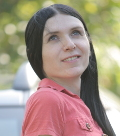
\includegraphics[height=68pt]{pic}}
    \end{minipage}
    \break
  \end{flushright}
\end{figure}


% ===== Skills ======
%

{\large \textbf{S}ummary}\\

\textbf{I}'m a software engineer with {\textbf {\small{10+}} years of experience working in research and commercial
conexts of both large and small companies. I build useful software by developing functional and correct
components, assembling them, releasing early. Experienced with modern front-end software design as well as
user interface and server side development.  \\\bigskip

%
% ===== Technical Skills =====
%

{\large \textbf{S}kills \& Qualifications} \hfill \href{https://github.com/linuxenko}{github.com/linuxenko}

\begin{itemize}[itemsep=-2pt]
  \item \textbf{ember}.js, \textbf{angular}.js, \textbf{backbone}.js, \textbf{react}/redux.js spa frameworks.
    Test with \textbf{mocha}, \textbf{chai}, \textbf{sinon}, \textbf{jsdom}, \textbf{jest}, coverage reporting with \textbf{istanbull} and, of course,
    \textbf{commonjs} helpers such as \textbf{browserify}, \textbf{webpack} and \textbf{babel}'s jsx transpiller, build tools.

  \item Work with general \textbf{css frameworks, pre/postprocessors},  \textbf{css degradation} strategies as
    well as \textbf{material} design and \textbf{mobile} web design principles.

  \item Experienced with \textbf{nodejs isomorphic} applications development, \textbf{REST}ful http API design, \textbf{websockets},
    basic \textbf{sql/nosql} database knowledge, \textbf{koa, express} nodejs frameworks.

  \item Deep knowledge of GNU/\textbf{Linux} administration and \textbf{bash} scripting/writing tests. Continuous integration: \textbf{jenkins, travis}. Vcs, mostly \textbf{git}, \textbf{vim} addicted user.

\end{itemize}

%
% ===== Education =====
%

{\large \textbf{E}ducation}

\begin{itemize}[itemsep=-2pt]
  \item \textbf{Kyiv Polytechnic Institute}, NTUU ``KPI'' \\
  Software Engineer (specialist degree) \hfill 2005-2010
\end{itemize}

%
% ===== Work Exp =====
%


{\large \textbf{W}ork Experience}

\begin{itemize}[itemsep=-2pt]

  \item \textbf{Dukascopy Bank SA}, Kiev, Ukraine\\
    Full-Stack Developer \hfill  2015 - 2016

  \item \textbf{Kaushan Media}, Kiev, Ukraine \\
    Front-End Developer \hfill  2014

  \item \textbf{BanQ Systems Ltd}, Kiev, Ukraine\\
    Full-Stack Developer \hfill  2013 - 2014

  \item \textbf{NavSystems Ukraine}, Kiev, Ukraine\\
    Java, Android, Javascript \hfill  2010 - 2012

  \item \textbf{Freelance},\\
    Java, Ruby on Rails, Javascript \hfill 2007-2010

  \item \textbf{WebGraFika P.E}, Simpferopol, Ukraine \\
    xhp, javascript \hfill 2005-2007

  \item \textbf{Trans-M Radio\texttrademark}, Simferopol, Ukraine \\
    Perl, C \hfill 2003-2005

\end{itemize}


%
% ===== Open Source =====
%

%{\Large \textbf{O}pen Source}
%
%\begin{itemize}[label=]
%  
%  \item \textbf{Webpack Configurator Web Application} \hfill\href{https://stuck.js.org}{https://stuck.js.org}
%  \begin{itemize}[label=-]
%    \item Webpack quick project creation GUI tool that guide you throught all \\
%  the options. Created for those who don't like spend time for project configuration.
%  \end{itemize}
%
%  \item \textbf{Unix Console Markdown Pager} \hfill\href{https://lessmd.js.org}{https://lessmd.js.org}
%  \begin{itemize}[label=-]
%    \item Minimal marked based unix terminal document viewer/pager with many\\
%  features like markdown to terminal translation, file change watching and more.
%  \end{itemize}
%
%  \item \textbf{Conceptual Design of Mobile Things} \hfill\href{http://codepen.io/linuxenko}{http://codepen.io/linuxenko}
%  \begin{itemize}[label=-]
%    \item Implementation of the creative ideas on the ``paper''. Different mobile\\
%    related things such as design, behavior of different components.\\\medskip
%  \end{itemize}
%
%
%\end{itemize}

%
% ==== Preferred technologies ====
%

%{\Large \textbf{C}urrent Stack} 

%\begin{itemize}[label=]
%  \item \textbf{Programming}: es6, ember, webpack, babel, npm, react, redux, jest, node, express\\
%  \textbf{Tools}: vim, bash, docker, travis ci, jenkins, hreoku, phantomjs+casper, systemd, git\\
%  \textbf{OS}: Linux
%\end{itemize}

% {\Large \textbf{D}sdsfsfsdsdfgsdf}

% \begin{multicols}{6}
%   \begin{itemize}[label=-]
%     \setlength\itemsep{-5pt}
%     \item react
%     \item es6
%     \item npm
%     \item linux
%     \item node
%     \item ember
%     \item sass
%     \item less
%     \item css
%     \item redux
%     \item express
%     \item git
%     \item linux
%     \item webpack
%     \item docker
%     \item jest
%     \item jenkins
%     \item vim
%     \item mocha
%     \item systemd
%     \item rest
%     \item karma
%     \item rwd
%     \item[] \dots
%   \end{itemize}
% \end{multicols}

% \ \medskip

\vfill

\begin{center}
  \footnotesize{\textsf{\copyright} 2016 Svetlana Linuxenko}
\end{center}

\end{document}

